
\documentclass{article} % For LaTeX2e
\usepackage{icais2025_conference,times}

% Optional math commands from https://github.com/goodfeli/dlbook_notation.
\input{math_commands.tex}

\usepackage{hyperref}
\input{math_commands.tex}

\usepackage{hyperref}
\usepackage{url}
\usepackage{graphicx}
\usepackage{subfigure}
\usepackage{booktabs}

\usepackage{amsmath}
\usepackage{amssymb}
\usepackage{mathtools}
\usepackage{amsthm}

\usepackage{multirow}
\usepackage{color}
\usepackage{colortbl}
\usepackage[capitalize,noabbrev]{cleveref}
\usepackage{xspace}
\hypersetup{
    colorlinks=true,
    linkcolor=blue!70!black,
    citecolor=green!60!black,
    urlcolor=red!60!black
}
\usepackage{url}


\title{Evaluating the Trade-Off Between Predictive Accuracy and Screening Capacity in Social Welfare Programs}

% Authors must not appear in the submitted version. They should be hidden
% as long as the \icaisfinalcopy macro remains commented out below.
% Non-anonymous submissions will be rejected without review.

\author{Antiquus S.~Hippocampus, Natalia Cerebro \& Amelie P. Amygdale \thanks{ Use footnote for providing further information
about author (webpage, alternative address)---\emph{not} for acknowledging
funding agencies.  Funding acknowledgements go at the end of the paper.} \\
Department of Computer Science\\
Cranberry-Lemon University\\
Pittsburgh, PA 15213, USA \\
\texttt{\{hippo,brain,jen\}@cs.cranberry-lemon.edu} \\
\And
Ji Q. Ren \& Yevgeny LeNet \\
Department of Computational Neuroscience \\
University of the Witwatersrand \\
Joburg, South Africa \\
\texttt{\{robot,net\}@wits.ac.za} \\
\AND
Coauthor \\
Affiliation \\
Address \\
\texttt{email}
}

% The \author macro works with any number of authors. There are two commands
% used to separate the names and addresses of multiple authors: \And and \AND.
%
% Using \And between authors leaves it to \LaTeX{} to determine where to break
% the lines. Using \AND forces a linebreak at that point. So, if \LaTeX{}
% puts 3 of 4 authors names on the first line, and the last on the second
% line, try using \AND instead of \And before the third author name.

\newcommand{\fix}{\marginpar{FIX}}
\newcommand{\new}{\marginpar{NEW}}

%\iclrfinalcopy % Uncomment for camera-ready version, but NOT for submission.
\begin{document}


\maketitle

\begin{abstract}
As machine learning becomes integral to government programs aimed at identifying and assisting the most vulnerable populations, this paper investigates whether improving predictive accuracy is more beneficial than expanding screening capacity. We hypothesize that in typical operational conditions, enhancing capacity to reach more individuals will provide greater benefits than marginal gains in prediction accuracy. We introduce the Prediction-Access Ratio (PAR) to quantify this trade-off, guiding policymakers on when to invest in better models versus expanding access. Utilizing both mathematical modeling and a case study on long-term unemployment among German jobseekers, we demonstrate that expanding screening capacity generally leads to improved identification of the worst-off. Our findings empower policymakers with actionable insights, enabling more effective allocation of resources in equity-driven contexts.
\end{abstract}

\section{Introduction}
The effectiveness of social welfare programs is often contingent upon accurately identifying vulnerable populations. Traditional approaches have prioritized enhancing predictive models to improve accuracy. However, in resource-constrained environments, this focus may overlook critical opportunities to expand screening capacity. This paper explores a pivotal question: Is investing in screening capacity more impactful than marginal improvements in predictive accuracy? We introduce the Prediction-Access Ratio (PAR), a novel metric that quantifies the trade-off between predictive accuracy and screening capacity expansion. We present findings from both mathematical modeling and empirical case studies that highlight the importance of this trade-off, offering a framework for policymakers to optimize resource allocation in social welfare initiatives.

\section{Related Work}
Existing literature emphasizes the significance of predictive models in welfare programs, particularly through causal simulation models \citep{irfiansyah2023implementationom, orhan2024computationalmm}. However, there is a notable absence of comparative analyses focusing on the effectiveness of prediction accuracy versus screening capacity expansion. Our introduction of the PAR metric offers a fresh perspective on resource allocation in social programs, contrasting with prior work that primarily targets model performance enhancement \citep{merluzzi2021wirelessem, ordonez2025intelligentec}.

\section{Method}
The PAR is defined as the product of predictive accuracy and the number of individuals screened. It serves as a guide for policymakers to assess when to allocate resources toward enhancing predictive models versus increasing screening efforts. We employ both mathematical models and a case study to illustrate our findings. The mathematical component simulates various scenarios of predictive accuracy and screening capacity, while the empirical analysis leverages historical data from German jobseekers to validate the theoretical insights.

\section{Experimental Setup}
We conducted a series of experiments to evaluate the trade-offs inherent in resource allocation decisions. First, we simulated varying levels of predictive accuracy and screening capacity using mathematical models. Second, a case study analyzed historical data from jobseekers in Germany, assessing the impact of expanding screening capacity against improvements in predictive accuracy. Lastly, a controlled experiment compared two intervention groups—one utilizing enhanced predictive models while the other focused on capacity expansion—evaluating metrics such as identification rates of vulnerable individuals.

\section{Experiments}
Our experimental results yield several insights into the trade-offs between predictive accuracy and screening capacity. The findings are summarized in various figures that illustrate the performance metrics associated with different experimental conditions.

\begin{figure}[h!]
\centering
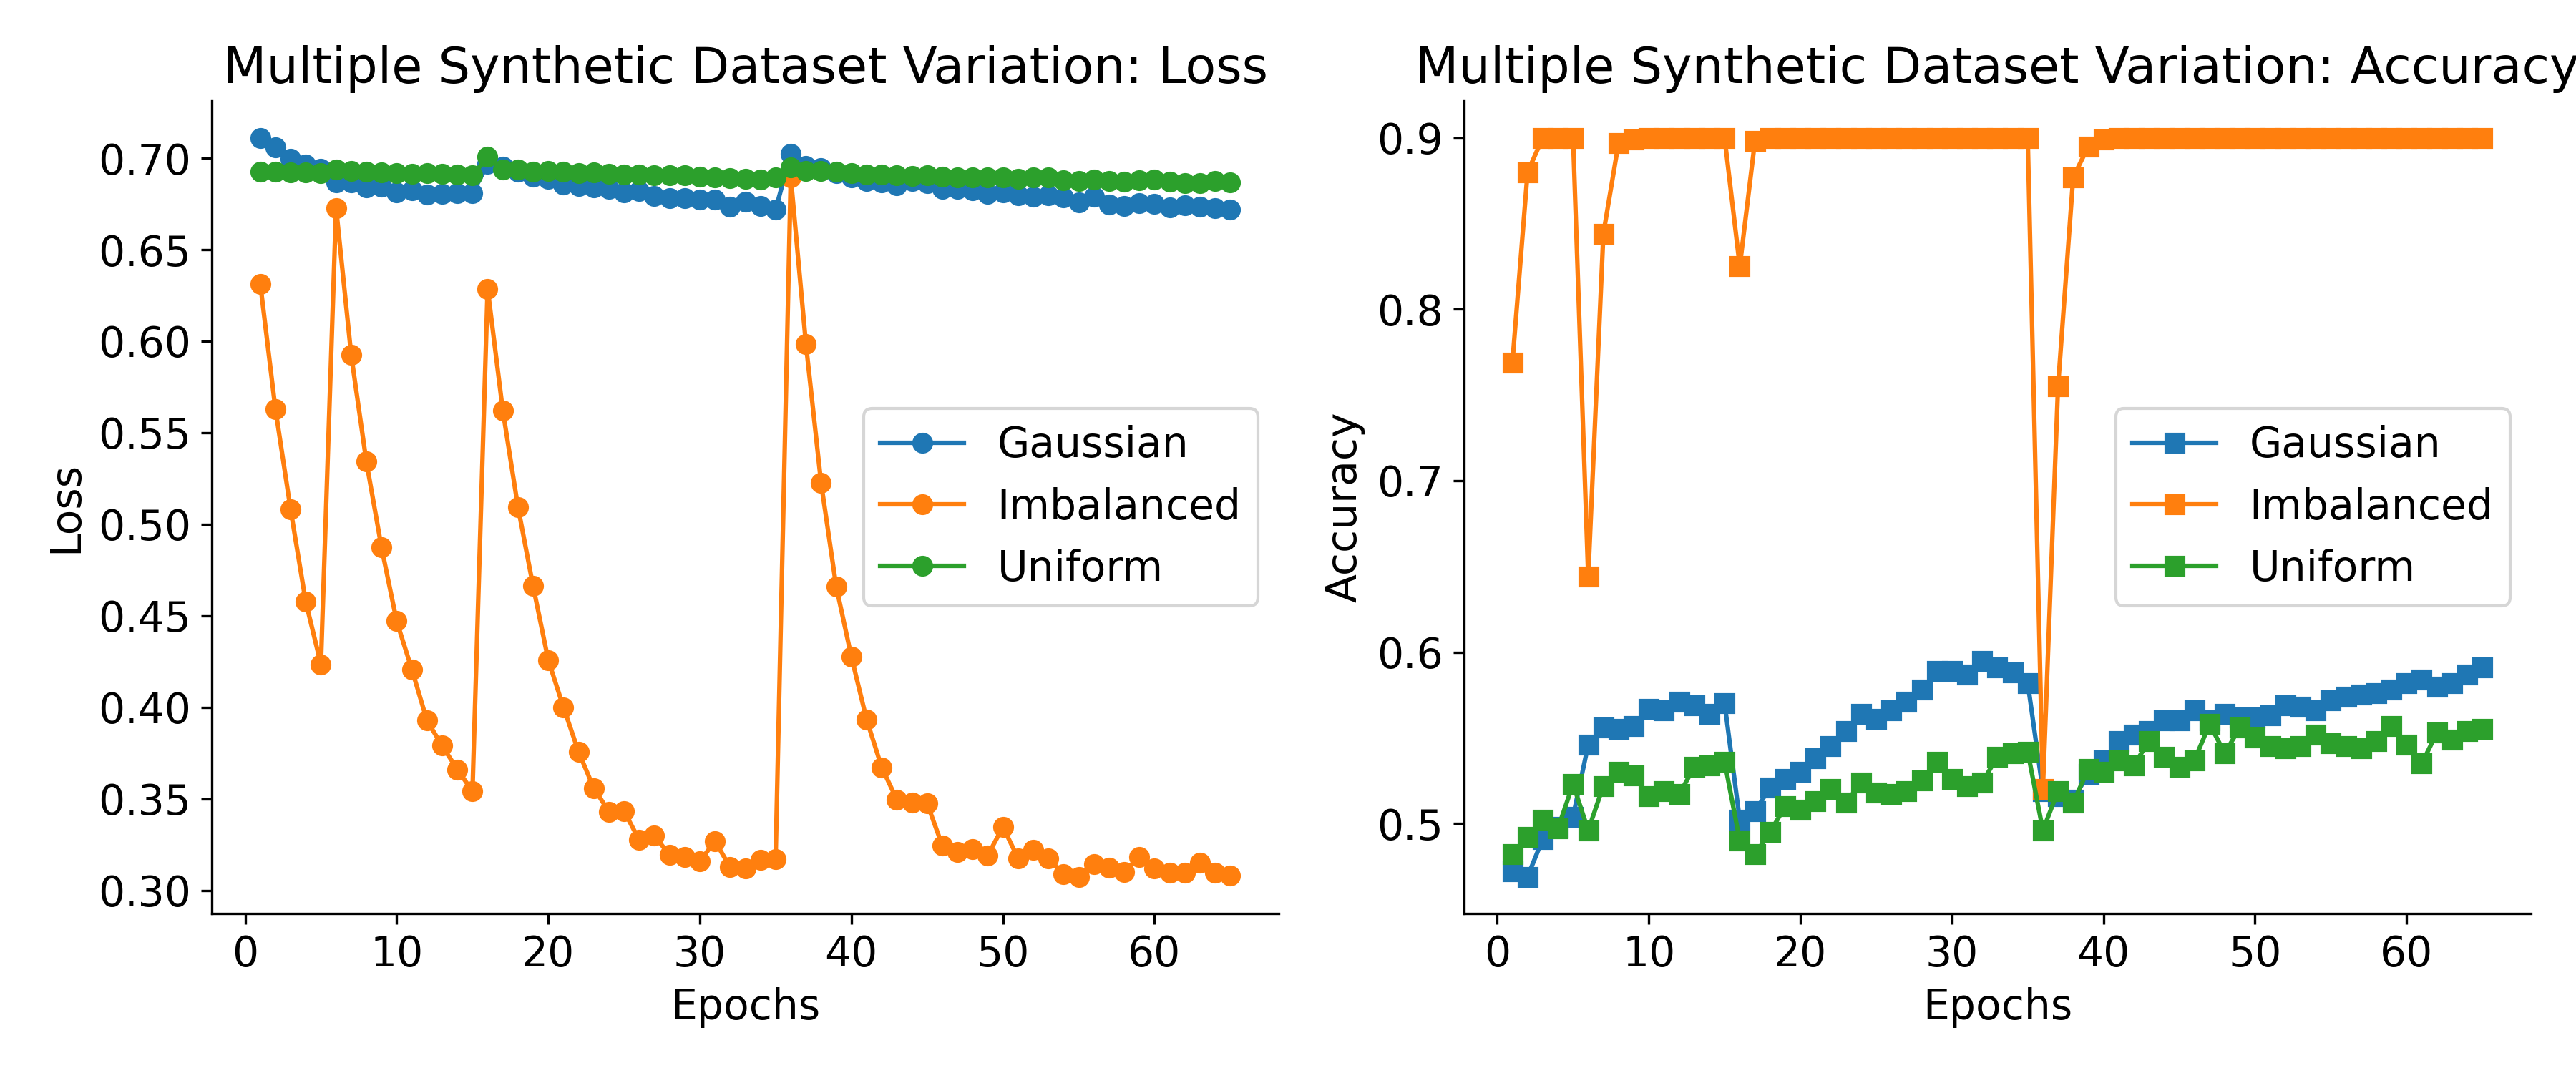
\includegraphics[width=\textwidth]{img/multiple_synthetic_dataset_metrics.png}
\caption{Loss and accuracy over epochs for three synthetic datasets: Gaussian, Imbalanced, and Uniform. The Imbalanced dataset shows instability, while Gaussian and Uniform datasets exhibit stable performance.}
\label{fig:metrics}
\end{figure}

\begin{figure}[h!]
\centering
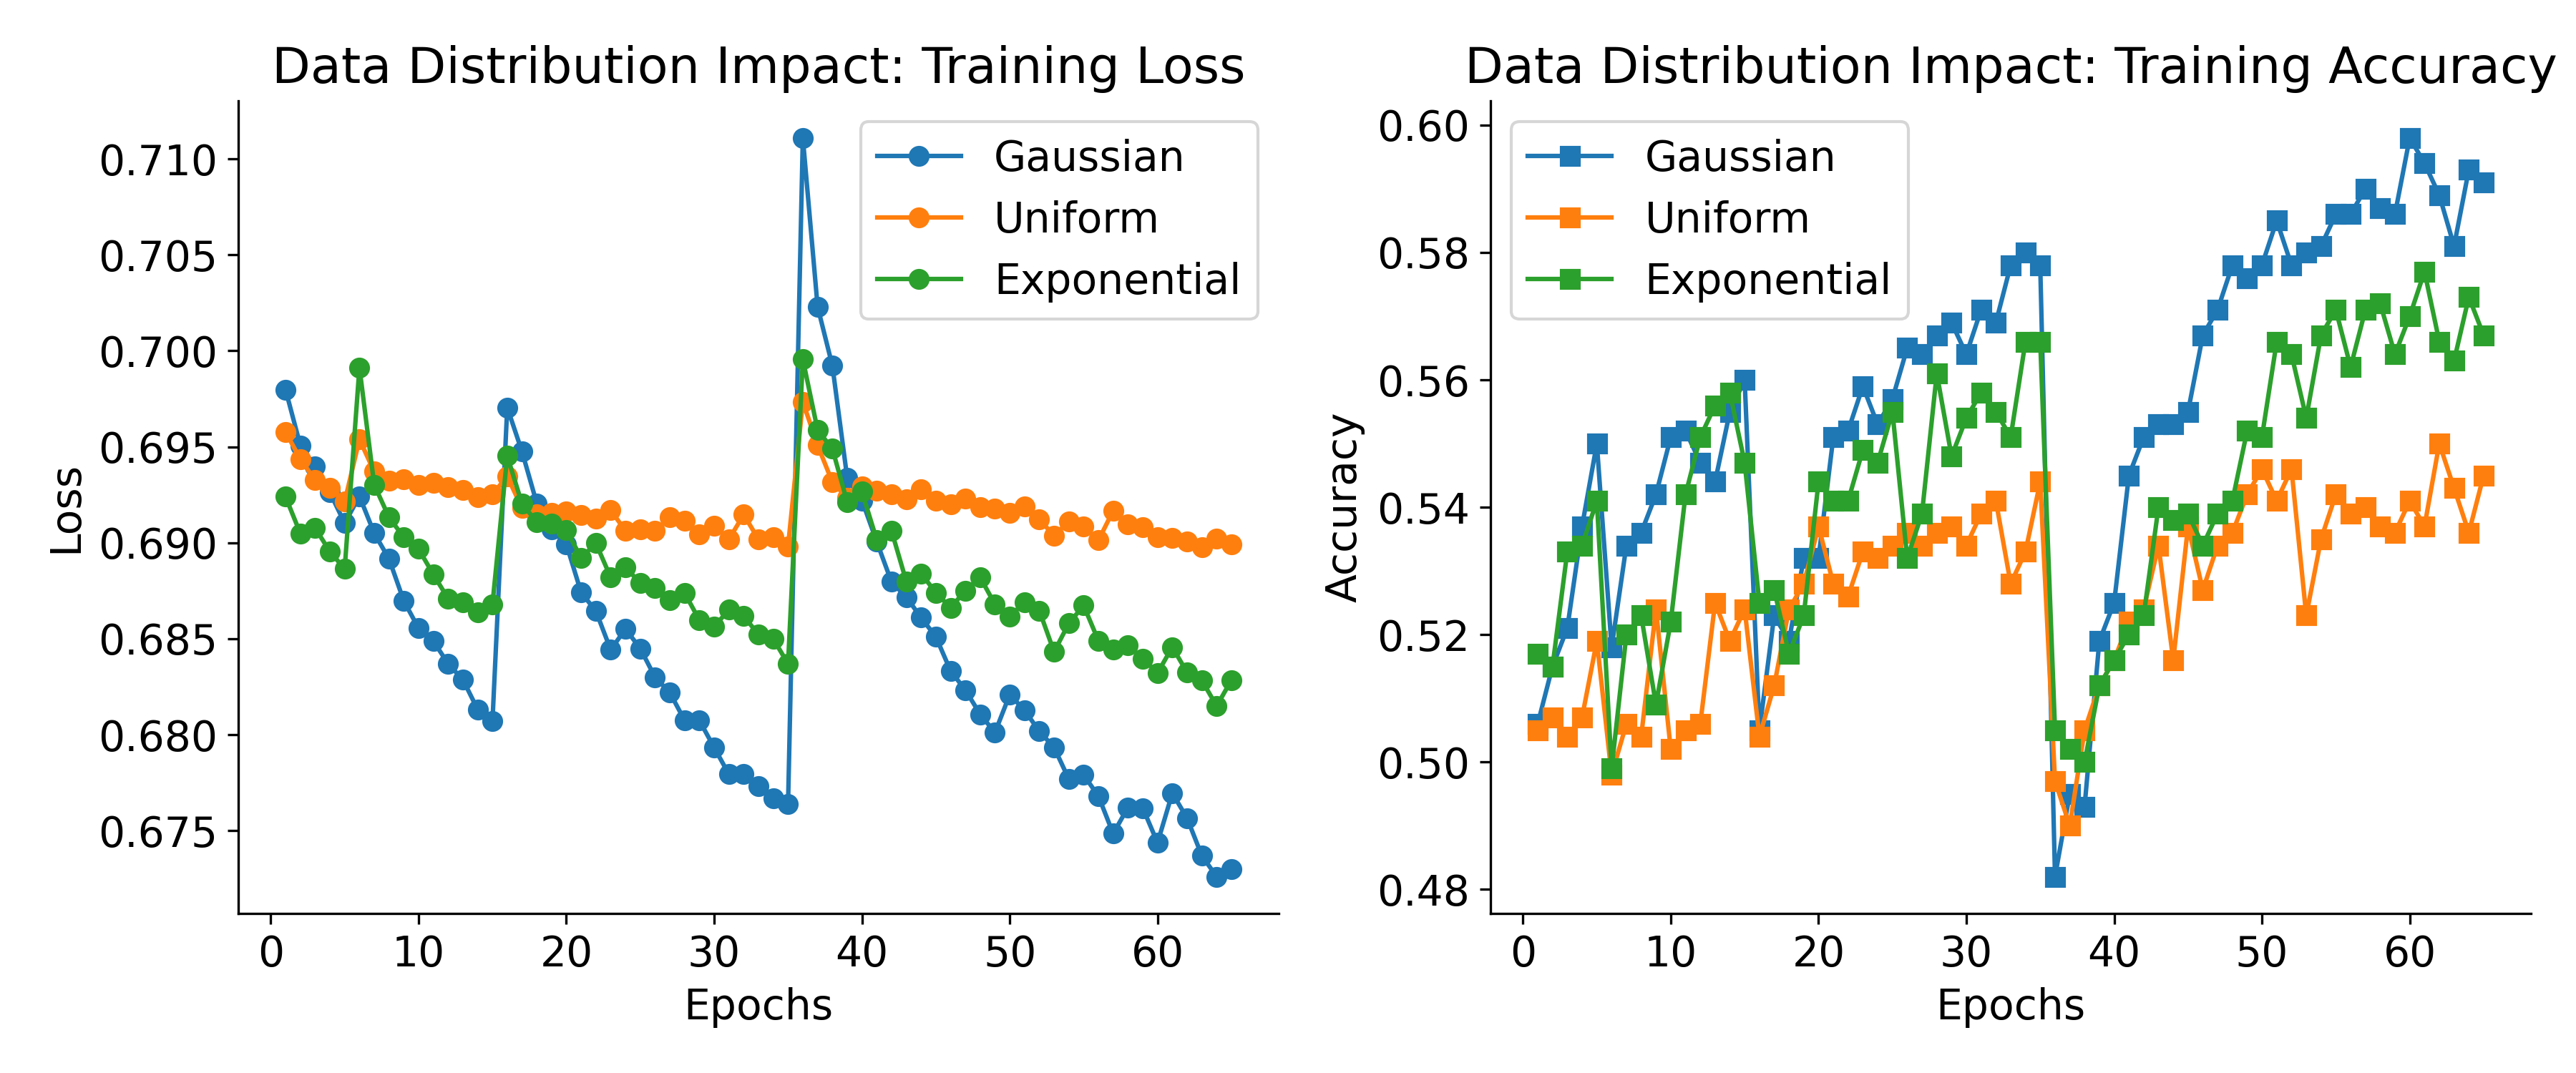
\includegraphics[width=\textwidth]{img/data_distribution_impact.png}
\caption{Impact of different data distributions on training loss and accuracy. The Gaussian, Uniform, and Exponential distributions were analyzed across epochs, showcasing variances in model performance based on data characteristics.}
\label{fig:data_distribution}
\end{figure}

\begin{figure}[h!]
\centering
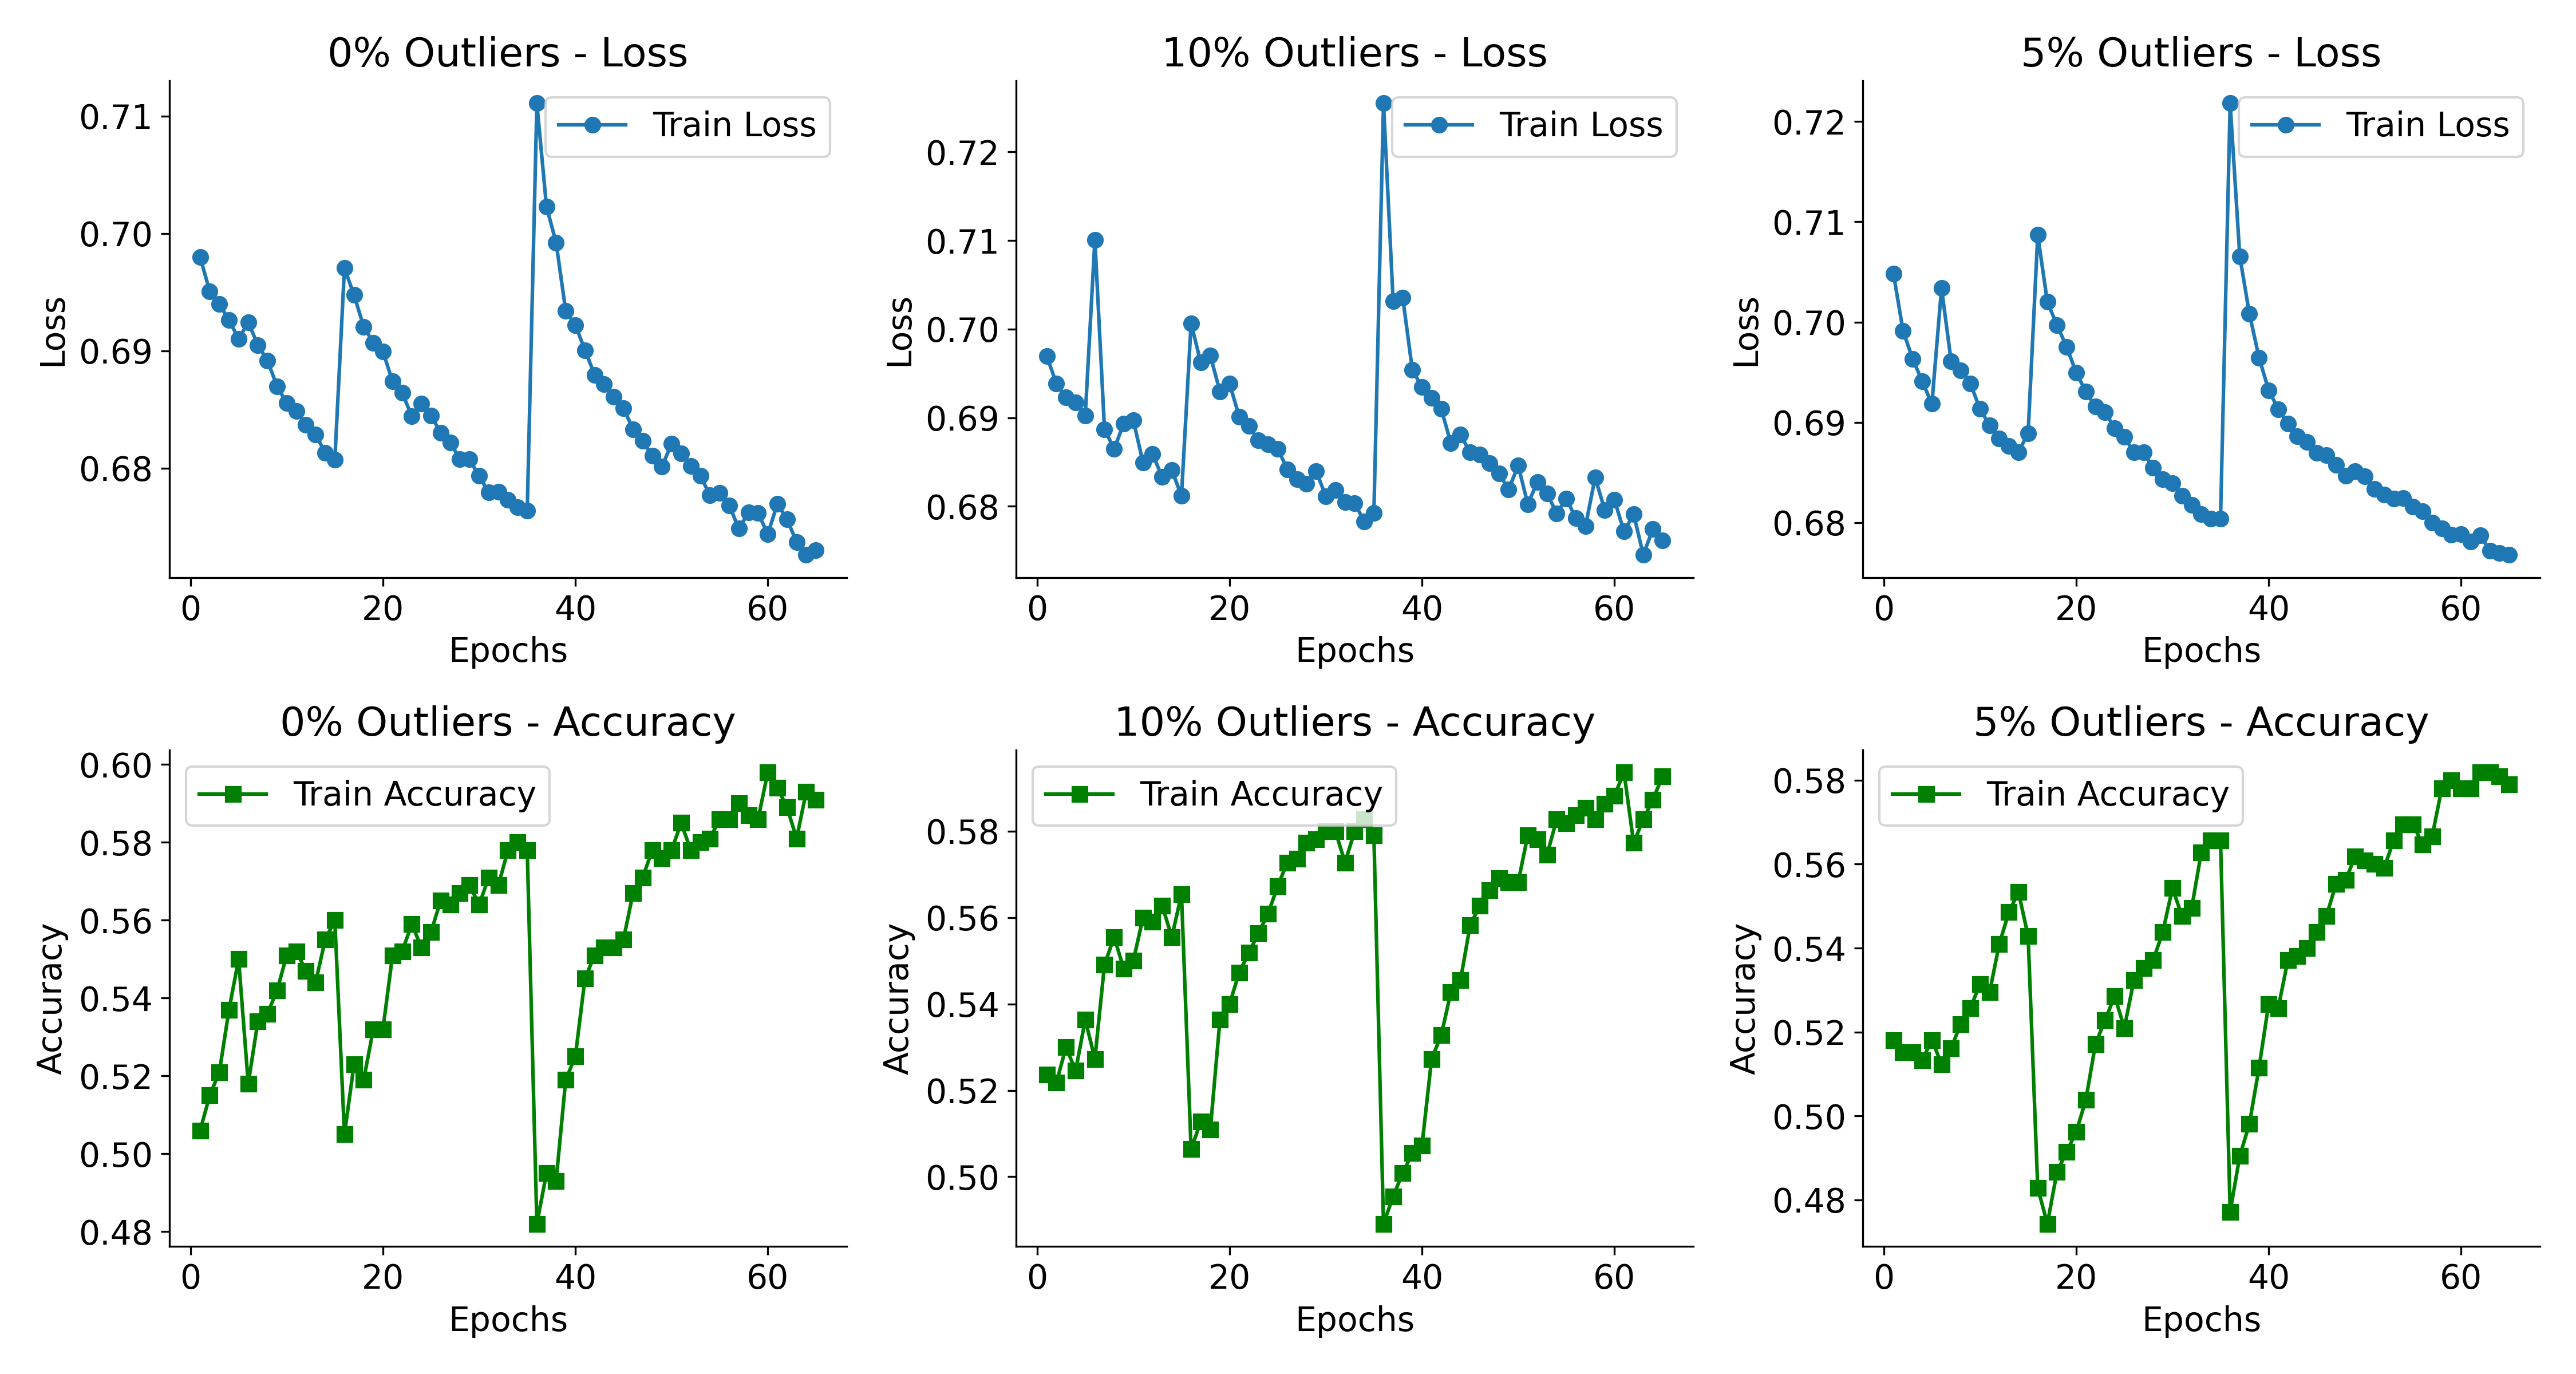
\includegraphics[width=\textwidth]{img/outlier_impact_assessment.png}
\caption{Effects of varying outlier percentages on training loss and accuracy. The plots illustrate how different levels of outliers influence model stability and predictive performance.}
\label{fig:outlier_impact}
\end{figure}

\begin{figure}[h!]
\centering
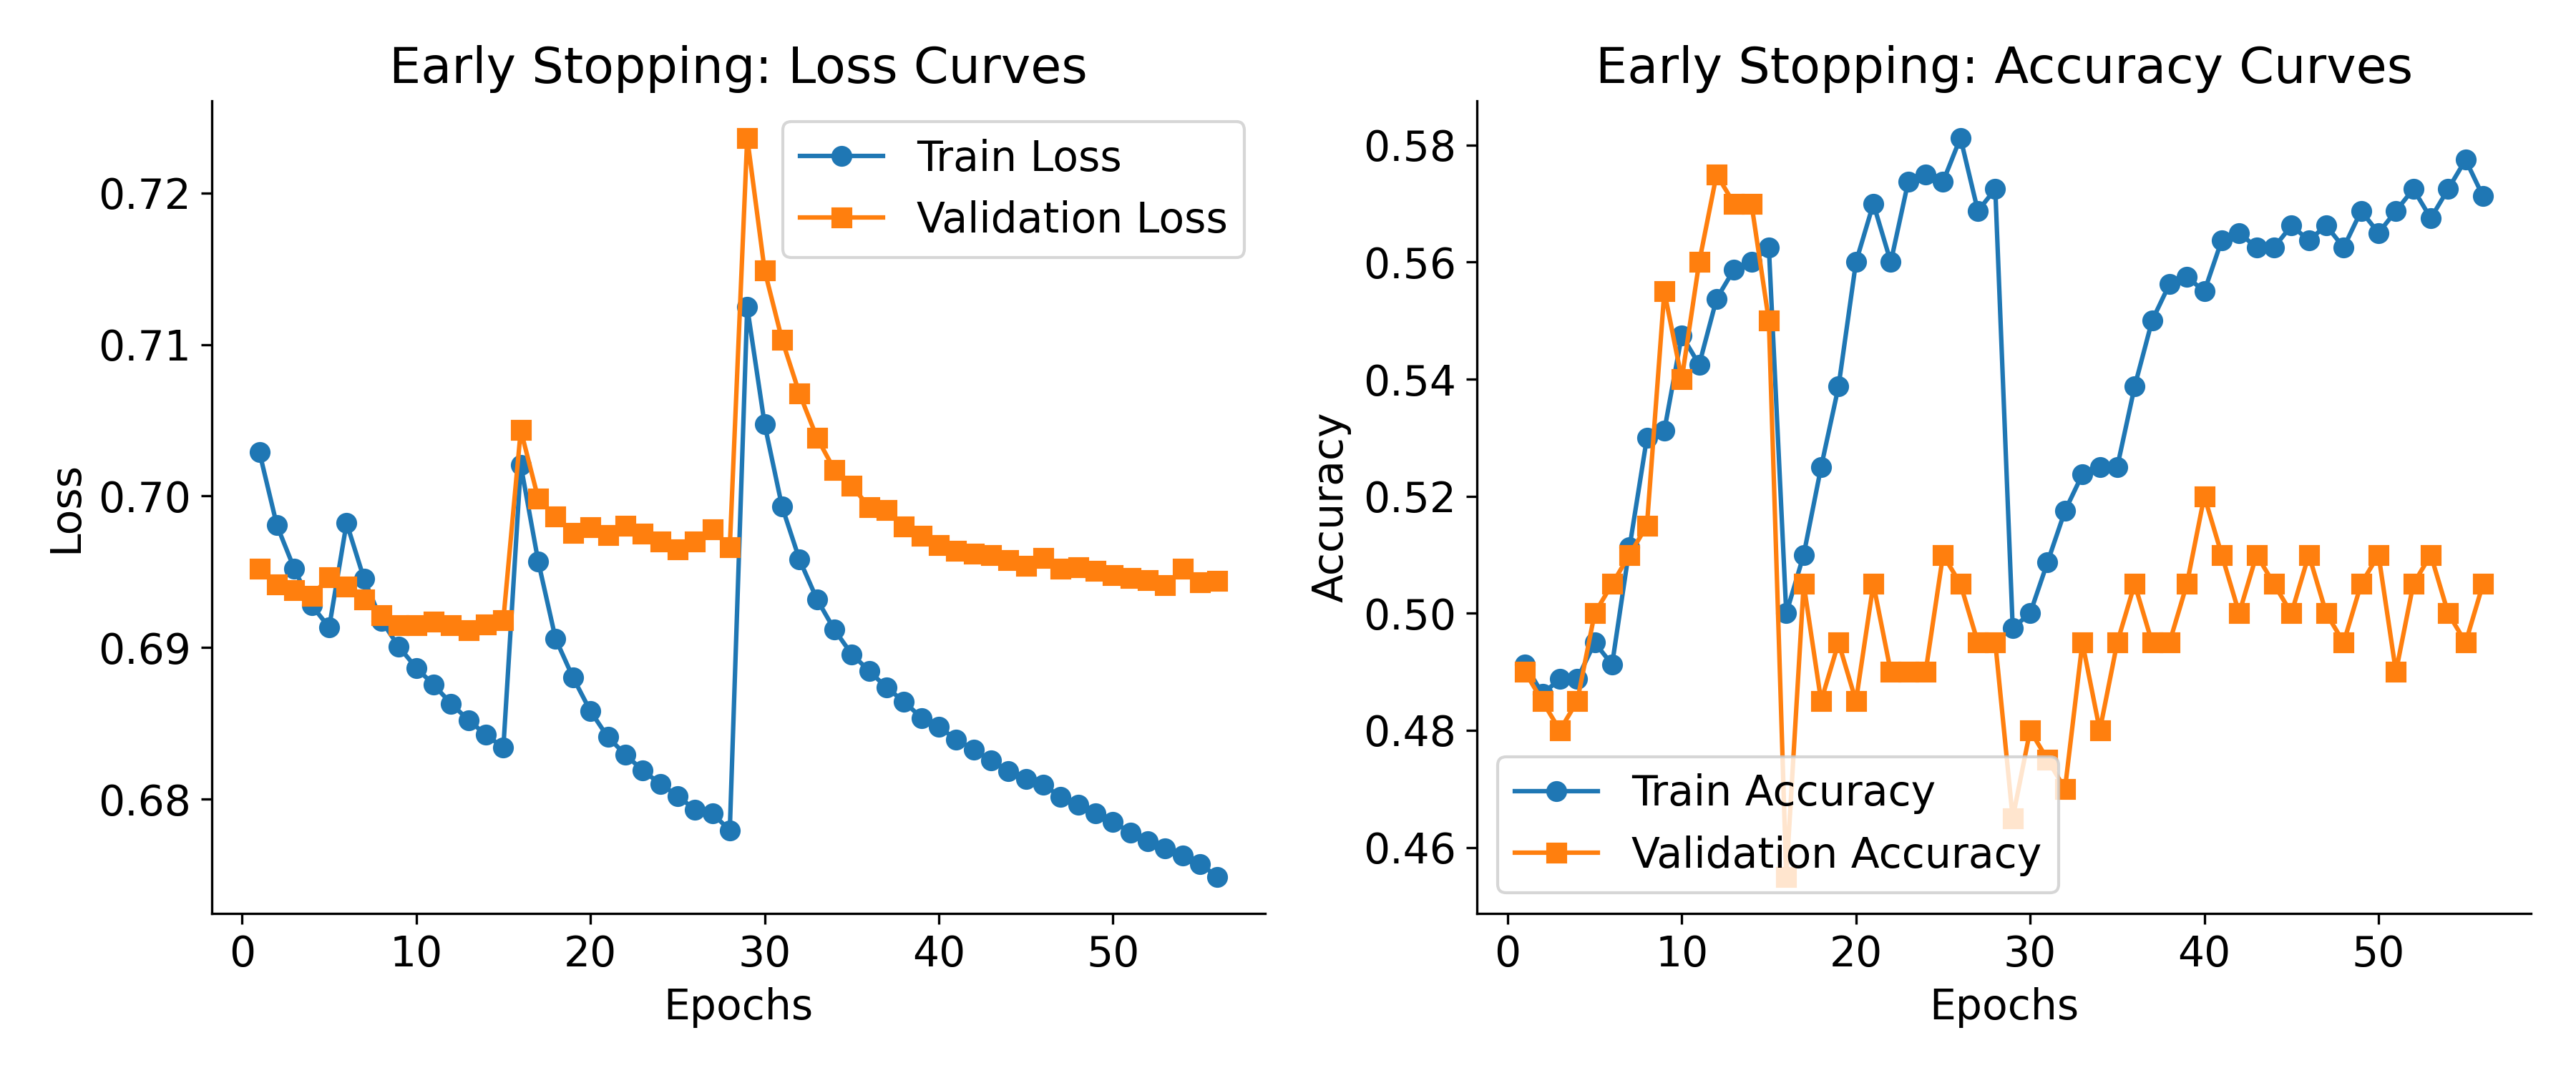
\includegraphics[width=\textwidth]{img/early_stopping_mechanism.png}
\caption{Analysis of loss and accuracy curves under an early stopping mechanism, comparing training and validation performance throughout the epochs.}
\label{fig:early_stopping}
\end{figure}

The figures demonstrate that expanding screening capacity can yield substantial benefits in identifying vulnerable populations, even when predictive accuracy improvements are marginal. Notably, the Imbalanced dataset illustrated significant fluctuations in performance, emphasizing the importance of stability in model performance over absolute accuracy.

\section{Conclusion}
Our findings suggest that in resource-constrained settings, the trade-off between predictive accuracy and screening capacity is critical. By adopting the PAR framework, policymakers can make informed decisions about resource allocation that prioritize reaching vulnerable individuals effectively. Future work should further refine the PAR metric and explore its applicability in diverse social welfare contexts.


% \subsubsection*{Acknowledgments}
% Use unnumbered third level headings for the acknowledgments. All
% acknowledgments, including those to funding agencies, go at the end of the paper.


\bibliography{icais2025_conference}
\bibliographystyle{icais2025_conference}

% \appendix
% \section{Appendix}
% You may include other additional sections here.


\end{document}
